\documentclass{article}
\usepackage[utf8]{inputenc}
\usepackage{graphicx}
\usepackage{hyperref}
\title{Probabilidad y Estadística con Numpy}
\author{Rodrigo Reyes M.}

\begin{document}

\maketitle

\section{Introducción a la probabilidad}

Este es un pequeño documento para recordar las nociones de probabilidad y estadística tipicamente vistas en la licenciatura.

Existen 3 axiomas principales postulados por el matemático ruso Kolmogorov:

\begin{enumerate}
\item La probabilidad siempre es expresada en un número real mayor o igual a cero y menor o igual a uno.
$$ 0 \leq P(A) \leq 1 $$
\item La probabilidad de el espacio muestral es uno.Es decir no hay eventos ajenos al espacio muestral.
$$ P(\Omega) = 1 $$
\item La probabilidad conjunta (o la unión) de eventos mutuamente exclusivos o ajenos es la suma de sus probabilidades.
$$ P(E_1 \cup E_2 \cup ..) = \sum_{i=1}^{\infty} P(E_i) $$
\end{enumerate}

Además de los axiomas de Kolmogorov hay dos conceptos muy importantes.

Dos eventos son ajenos o independientes si su probabilidad no influye en la probabilidad del otro.

Ejemplos:
\begin{itemize}
\item Lanzar una moneda no afecta la probabilidad de obtener 6 en un dado por tanto son eventos independientes
\item Si saco una pelote roja de una urna con 2 pelotas rojas y 100 negras la probabilidad de obtener nuevamente una pelota roja es menor por tanto NO SON EVENTOS INDEPENDIENTES.
\item Aunque paresca poco intuitivo el haber obtenido 7 caras en una serie de lanzaminetos de moneda NO AFECTAN la probabilidad de obtener nuevamente cara por tanto son independientes.
\end{itemize}

\section{Ejercicios}

\begin{enumerate}
\item Si P(A) = 0.4 ¿Cuál es la probabilidad de $ \neg P(A) $ ?
\item De los siguientes eventos indique con la letra I si son independientes y X si no lo son.
\begin{itemize}
\item La probabilidad de obtener un rey de corazones si obtuve un rey de tréboles.
\item  La probabilidad de obtener una reina de espadas si obtuve un 3 de corazones.
\item La probabilidad de que llueva si me gané la lotería.
\end{itemize}

\item Tenemos una urna con 5 pelotas de la siguiente forma, 2 son rojas , otras 2 son verdes y 1 es negra. Si realizo dos experimentos en donde saco una pelota y la vuelvo a insertar en la urna para sacar nuevamente una pelota.¿Cuál es la probabilidad de obtener una pelota negra?


\end{enumerate}


\section{Introducción a Numpy y Python}
Python es un lenguaje interpretado con Orientación a Objetos creado por Guido van Rossum.En éste curso utilizaremos la biblioteca de Numpy que es ampliamente utilizada para análisis numérico y minería de datos.

Las funciones en Python se definen de la siguiente forma


\begin{verbatim}
define fun():
    print("hola")
\end{verbatim}

El lenguaje Python utiliza Tabs o espacios para delimitar bloques de código, es decir identar en Python es equivalente a generar un bloque de \{ \} en Java.

Cabe destacar que es recomendable utilizar uno de los dos métodos y no ambos (es decir no mezclar Tabs y espacios).Algunos editores de texto convierten automáticamente las tabs en cuatro espacios.

Para éste curso se requiere instalar IPython que es una herramienta que simplifica mucho el análisis de datos.

Ésta herramienta al ser instalada con SciPy instala automáticamente las dependencias que nos permiten utilizar tanto Numpy como Matplotlib (una herramienta para generar gráficas).
\subsection{Funciones básicas de Numpy}

Para comenzar con los siguientes ejercicios deberás ejecutar el comando \begin{verbatim}
ipython --pylab
\end{verbatim}

Una vez iniciado el ambiente, ejecuta el siguiente comando.
\begin{verbatim}
random.random_sample()
\end{verbatim}

El objeto random tiene un método \verb#random_sample# que al ser llamado sin argumentos genera un número entre 0 y 1 de manera aleatoria.
(La muestra se toma de una distribución uniforme que se verá más adelante)

\subsection{Ejercicios de código}
\begin{enumerate}
\item Crea un archivo en el editor de tu preferencia que se llame \verb#proba.py#
\item En ése archivo crea la función \verb#lanzar_moneda# que retorne 0 si al llamar a \verb#random.random_sample()# el número es menor o igual a 0.5 y 1 en otro caso.
\item Carga el archivo \verb#proba.py# en IPython.
\item Revisa que puedas ejecutar \verb#lanzar_moneda()#
\item Modifica \verb#proba.py# ahora creando una funcion \verb#simular(n)# que simule lanzar la moneda n veces y regrese un arreglo con la primera posición indique la suma de veces que \verb#lanzar_moneda# regresó 0 y en la segunda posición la suma de veces que regresó 1.
\end{enumerate}
Tip:
Para crear un arreglo en Numpy se crea con el método array y con una tupla como argumento.
\begin{verbatim}
array([1,2,3]) # Arreglo con los elementos 1 , 2 ,3.
\end{verbatim}

\subsection{¡Vamos a graficar!}
Es hora de ver los resultados del pequeño simulador de lanzamiento de monedas que hemos creado.Muchas veces los ananlistas pueden deducir muchas propiedades sobre los datos al ser graficados.

La forma más sencilla de ver la información es mediante una gráfica de pastel o pie plot.

En IPython es extremadamente fácil crear uno.Simplemente ejecuta la siguiente linea de código.
\begin{verbatim}
pie([10,20,30])
\end{verbatim}
El resultado debe ser similar a la siguiente figura

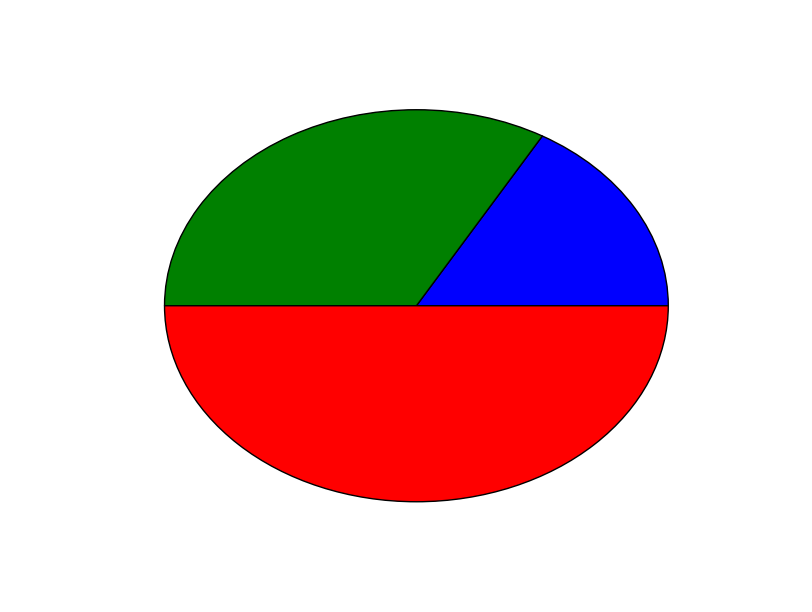
\includegraphics[width=4cm, height=4cm]{pastel_1.png}

Matplotlib permite modificar muchas cosas respecto a una gráfica desde los colores, las etiquetas e incluso hacer animaciones.

Si deseas saber más acerca de los parámetros que se pueden modificar el siguiente link te ayudará
\url{http://matplotlib.org/1.2.1/api/pyplot_api.html?highlight=hist#matplotlib.pyplot.pie}

\subsection{Ejercicios de código}
\begin{enumerate}
\item Modifica \verb#proba.py# creando una funcion \verb#graficar(n)# que muestre una gráfica utilizando a la n como parametro para la función \verb#simular(n)#.Es decir la gráfica de Pie debe mostrar la proporcion de cara o cruz en los lanzamientos virtuales de moneda.
\item Ejecuta la función \verb#graficar(5)#
\item Ejecuta la función \verb#graficar(10)#
\item Ejecuta la función \verb#graficar(10000)#
\end{enumerate}
\section{Estadística}
\subsection{Teorema de Límite Central}
Una de los pilares de la estadística moderna se centra en el Teorema de Límite Central.Formalmente nos dice:

Sea $(X_1,X_2, ...,X_n)$ un conjunto de variables aleatorias independientes e idénticamente distribuidas con media $\mu$ y varianza $0 < \sigma^2 < \infty $.Entonces para una n lo suficientemente grande la media se distribuye  normal con media $\mu$ y varianza $\sigma^2$. $$\bar{X} = \frac{1}{n}\sum_{i=1}^{n}X_i \sim N(\mu,\sigma^2)$$
Lo importante de el teorema es que nos permite que al tener una muestra grande modelamos utilizando la distribución normal o gaussiana cuyas propiedades son bien conocidas y ampliamente estudiadas.
\subsection{Ley de los grandes números}
Es importante conocer la relación entre la probabilidad y la estadística.En los ejercicios previos se pudo observar que las simulaciones computacionales pueden aproximarse a su probabilidad.
Por ejemplo la siguiente es una gráfica realizada a partir de una simulación de lanzamientos de dos dados.

\begin{figure}
\centering
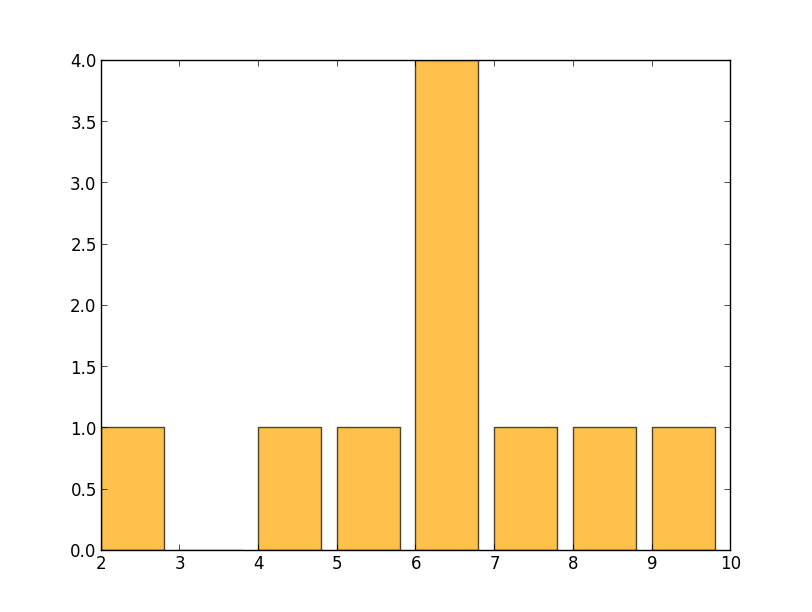
\includegraphics[width=7cm, height=7cm]{hist1.png}
\caption{Histograma de lanzamiento de dos dados con 10 experimentos}
\label{fig:my_label}
\end{figure}
\begin{figure}
\centering
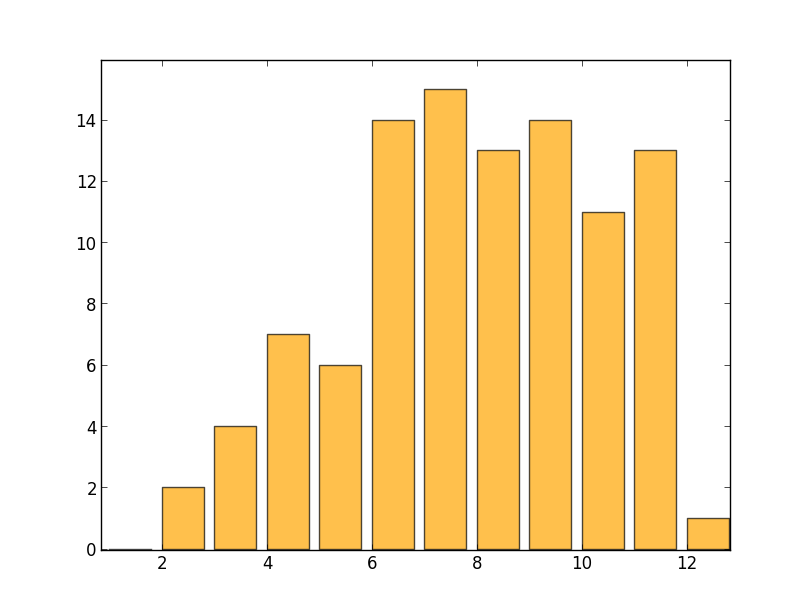
\includegraphics[width=7cm, height=7cm]{hist2.png}
\caption{Histograma de lanzamiento de dos dados con 100 experimentos}
\label{fig:my_label}
\end{figure}
\begin{figure}
\centering
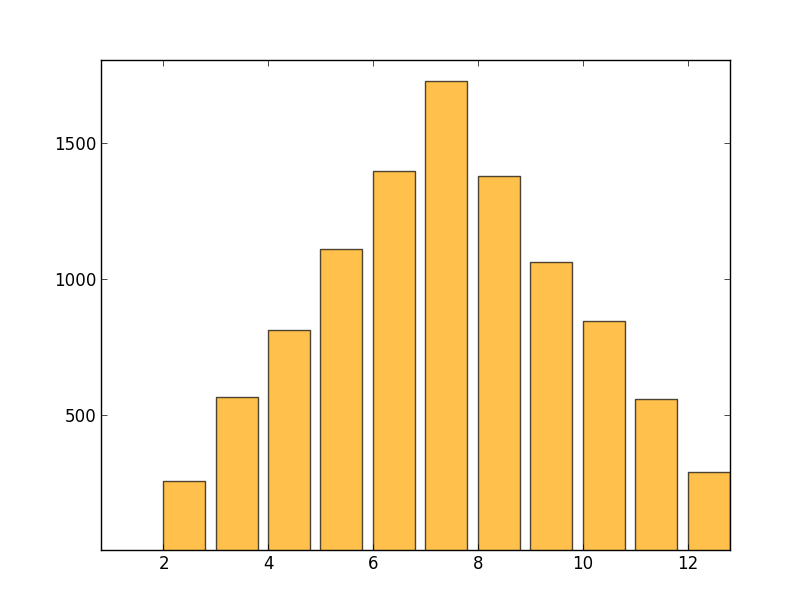
\includegraphics[width=7cm, height=7cm]{hist3.png}
\caption{Histograma de lanzamiento de dos dados con 10000 experimentos}
\label{fig:my_label}
\end{figure}
A este tipo de gráficos se les llama histogramas y nos muestra visualmente la distribución de los datos.
Se puede observar claramente que al realizar el experimento 10000 veces los datos toman una forma muy peculiar, similar a la de una campana.También es fácil ver que el 7 es el valor más común.Veamos que la probabilidad de obtener una suma de 7 al tirar dos dados es 0.16 y se obtuvieron aproximadamente 1740 sietes.Ésto nos dá una proporción de 0.174 que es un número muy cercano a 0.16.(Incluso se ejecutó una simulación con 10000000 de experimentos y se obtuvieron 167129 que es 0.167129 todavía más cercano a 0.16).Entonces formalmente la ley de grandes números nos dice (En este caso la ley fuerte, la ley débil es ligeramente distinta y se aplica en otros casos.)
$$ P(\lim_{n\to\infty} \bar{X} = \mu ) = 1 $$
Es decir la media muestral se parece cada vez más a la media global.
Incluso utilizando el teorema previo de límite central los datos se pueden modelar con una distribución normal con $ \mu = 7 $
Sin embargo, hay dos cosas importantes a destacar, como se puede ver en el histograma los datos no tenian una distribución aparente cuando el número de experimentos es pequeño.Ésto es de enorme importancia cuando se trabaja con datos debido a que se pueden cometer errores al tener conjuntos muy pequeños de datos que no representen correctamente al total de la población.Esto hay que tomarlo como pauta para el último tema que son las falacias estadísticas más comunes y cómo reducir o detectarlas.






\subsection{Falacias estadísticas}

Es importante poder identificar las falacias estadísticas.Una frase célebre de Mark Twain \textit{There are three kinds of lies: lies, dammed lies and statistics}, muchas veces la pseudociencia y algunas investigaciones mal hechas utilizan datos estadísticos como único sustento a teorías que no son las correctas.

La falacia más común es \textit{Correlación no implica causalidad}, esto intenta sustentar una generalización a partir de una correlación estadística.

Por ejemplo supógase que se realiza un estudio y se determina que estadísticamente los alumnos obtienen mejores calificaciones en el semestre cercano a el invierno.

De ésto se concluye que el aprendizaje está ligado a las estaciones o al clima.

Es fácil ver que a pesar que existe una aparente correlación no hay suficiente evidencia que permita sustentar que el invierno cause mejoría en los estudios.Bien se puede deber a otros factores \textit{escondidos o no aparentes}, tales como
\begin{enumerate}
\item El semestre es más corto por lo que las clases se reducen.
\item Los profesores tienden a ausentarse más debido a que hay mayor cantidad de fechas festivas.
\item etc..
\end{enumerate}
En muchos estudios serios se utilizan grupos de control para poder reducir conclusiones erróneas y sobretodo se hace mención de el error que tienen las mediciones y la magnitud de los muestreos.

Otra falacia muy común es comunmente vista con una anécdota.
Un turista visita Texas y descubre que en un granero hay una serie de circulos concéntricos de color rojo y blanco a manera de objetivos.Y en cada uno de los círculos hay un agujero causado por una bala.El turista inmediatamente felicita al granjero que porta un rifle suponinedo que resulta ser un experto en tiro al blanco, mientras su esposa le dice \textit{En relidad es muy malo en tiro al blanco, sin embargo es muy bueno pintando blancos en los hoyos que dejan las balas.}
Ésta falacia se debe a que amoldamos las teorías ó hipótesis para que embonen con los datos.




\subsection{Ejercicios}
\begin{enumerate}
\item Investiga la función de densidad para la distribución normal o gaussiana.
\item ¿Que significa $\mu$ y $\sigma$ ? (En la función de densidad normal)
\item ¿Qué es la desviación estándar?¿Cómo está relacionada con la varianza?
\item Encuentra o inventa una falacia estadística.Describe ¿porqué es falacia?
\end{enumerate}




\subsection{Ejercicios de código}
\begin{enumerate}
\item Crea una simulación de una urna con 5 pelotas: 2 rojas, 2 verdes y una negra.Tal cómo se describe en el ejercicio 3 de la sección 2.
\item Realiza la simulación 10000 veces y grafica el resultado en un gráfico de pastel con los colores correspondientes a el color de las pelotas.
\item Indica la proporción que se obtuvo.¿Qué tan cercana es a el resultado que se obtuvo utilizando probabilidad?¿Porqué?


\end{enumerate}


\end{document}
